\chapter{Problematyka wirtualnej rzeczywistości}
\label{ch:zagadnienia}
Zanim zostanie przedstawione wykonanie projektu, należy zapoznać się z podstawowymi zagadnieniami związanymi ze światem technologii wirtualnej rzeczywistości oraz sposobem w jaki świat ten wchodzi w interakcję z użytkownikiem. W tym celu zostanie pokazane czym jest wirtualna rzeczywistość, w jaki sposób producenci zestawów VR (ang. Virtual Reality) podchodzą do tematu kontrolerów oraz jak narodził się pomysł na rękawice-kontroler, która pewnego dnia może zastąpić wykorzystywane do tej pory rozwiązania. 
	\section{Czym jest wirtualna rzeczywistość?}
	\label{sec:vr}
	Przede wszystkim przed rozpoczęciem pracy nad kontrolerem należy zrozumieć czym jest wirtualna rzeczywistość oraz jak wygląda interakcja pomiędzy światem rzeczywistym a wirtualnym. Rzeczywistość wirtualna jest to wygenerowany komputerowo trójwymiarowy obraz przedstawiający pewną scenę w której mogą być umiejscowione różne obiekty imitujące przedmioty, ludzi, zdarzenia oraz interakcje pomiędzy nimi. W zależności od sposobu stworzenia takiej przestrzeni użytkownik może się w tej przestrzeni poruszać, bądź zostać ustawiony w jednym punkcie. Scena to może zawierać elementy zarówno prawdziwego jak i fikcyjnego świata. Niezależnie jednak od sposobu prezentacji, założeniem świata wirtualnego jest stworzenie naturalnych i realnych doznań. Realność jest odbierana przez ludzki mózg jako seria sygnałów pochodzących z różnych zmysłów, dzięki którym możemy określić czy środowisko w jakim się znajdujemy jest tym ``realnym", które znamy z życia codziennego. W związku z tym aby w pełni oszukać ludzki mózg, nawet najmniejsze detale muszą odwzorowywać dokładnie elementy świata rzeczywistego, co ludzkość stara się osiągnąć poprzez wprowadzanie ciągłych udoskonaleń technologicznych. Najważniejszym elementem prezentowania wirtualnej rzeczywistości było wprowadzenie okularów VR, które całkowicie blokowały świat zewnętrzny, pozwalając jedynie na rozglądanie się w świecie stworzonym przez twórców. Typowym elementem jest możliwość rozglądania się w świecie wirtualnym dzięki poruszaniu głową, dzięki czemu obraz generowany i wyświetlany w okularach niejako pokazuje świat wirtualny w ten sam sposób jak odkrywamy świat rzeczywisty. Ważnym elementem w tworzeniu światów wirtualnych jest poznanie fizjonomii człowieka. Obraz który widzi człowiek jest jedynie częścią otoczenia - równie ważny jest zmysł słuchu który niejako potwierdza widziany przez użytkownika obraz w postaci sygnałów dźwiękowych, których osoba się spodziewa widząc dany przedmiot. Jeżeli sygnały są sprzeczne, długotrwałe użytkowanie takiego sprzętu potrafi doprowadzić do znanej wielu osobom choroby lokomocyjnej. Mając do dyspozycji obraz oraz dźwięk twórcy mogą tworzyć różnego rodzaju pokazy oraz filmy $360^o$, dzięki czemu odbiorcy otrzymują informacje w nowy ciekawy sposób. Oczywiście w pewnym momencie prezentowanie obrazu nie było wystarczające - w celu podniesienia poziomu realności widzianego obrazu, użytkownik powinien móc wchodzić w interakcję z obiektami wokół niego się znajdującymi. Najprostszym zastosowanym rozwiązaniem jest dodanie przycisku oraz celownika na środku widzianej przez użytkownika sceny. Dzięki temu gdy wycelowano w dany obiekt, przycisk służył niejako mysz komputera pozwalając na wywołanie zaprogramowanej akcji obiektu. W skomplikowanych przedsięwzięciach tak prosta obsługa nie jest jednak wystarczająca, w związku z czym zostały stworzone kontrolery z których pomocą można było wchodzić w interakcję w świecie wirtualnym~\cite{vrHistory}. 

\section{Działanie kontrolerów w VR}
\label{sec:kontroleryVR}
Pomiędzy kontrolerami typu gamepad, używanych do gier wideo oraz tymi używanymi do interakcji z obiektami wirtualnej rzeczywistości jest kilka różnic zarówno z wewnątrz jak i zewnątrz. Podstawowe założenie obu jest jednak takie samo, ponieważ muszą one spełnić te same funkcje niezależnie od sposobu prezentacji obrazu użytkownikowi. Często spotykaną praktyką jest umiejscowienie na kontrolerze pewnego rodzaju joysticka pozwalającego na ruch oraz przyciski dzięki którym można wykonywać akcje zależne od środowiska w jakim się znajduje użytkownik. Oczywiście sposób obsługi nie jest taki sam. Wyświetlając obraz na ekranie kontroler zazwyczaj jest obsługiwany oburącz w związku z czym w ten sposób też są one projektowane - stąd pojawiają się pierwsze różnice wizualne. Kontrolery w świecie VR przede wszystkim są projektowane tak aby były obsługiwane jedną ręką. Oprócz tego zazwyczaj posiadają pewnego rodzaju system śledzenia wewnętrzny, zewnętrzny bądź łączący oba, aby można było określi pozycję kontrolera w przestrzeni, dzięki czemu pozycję kontrolerów można odwzorować w świecie wirtualnym np. jako dłonie. Sprawia to jednak że posiadają one często dodatkowe, nietypowo wyglądające elementy. Śledzenie kontrolerów w przestrzeni nie należy do problemów dających się łatwo rozwiązać w związku z czym wiele firm zdecydowało się na różne sposoby rozwiązania tego zadania. Pomimo braku śledzenia, gamepady takich firm jak Sony czy Microsoft współpracują z technologiami VR na konsole przez nich produkowane, jednak zagłębienie się w świat wirtualny nie jest tak łatwe jak w przypadku kontrolerów do tego przeznaczonych. Na zdjęciu~\ref{fig:kontrolery} znajdują się przykładowe kontrolery dwóch znanych producentów na rynku - HTC Vive oraz Oculus Rift.
\begin{figure}[h]
\centering
	\begin{subfigure}[b]{0.45\textwidth}
	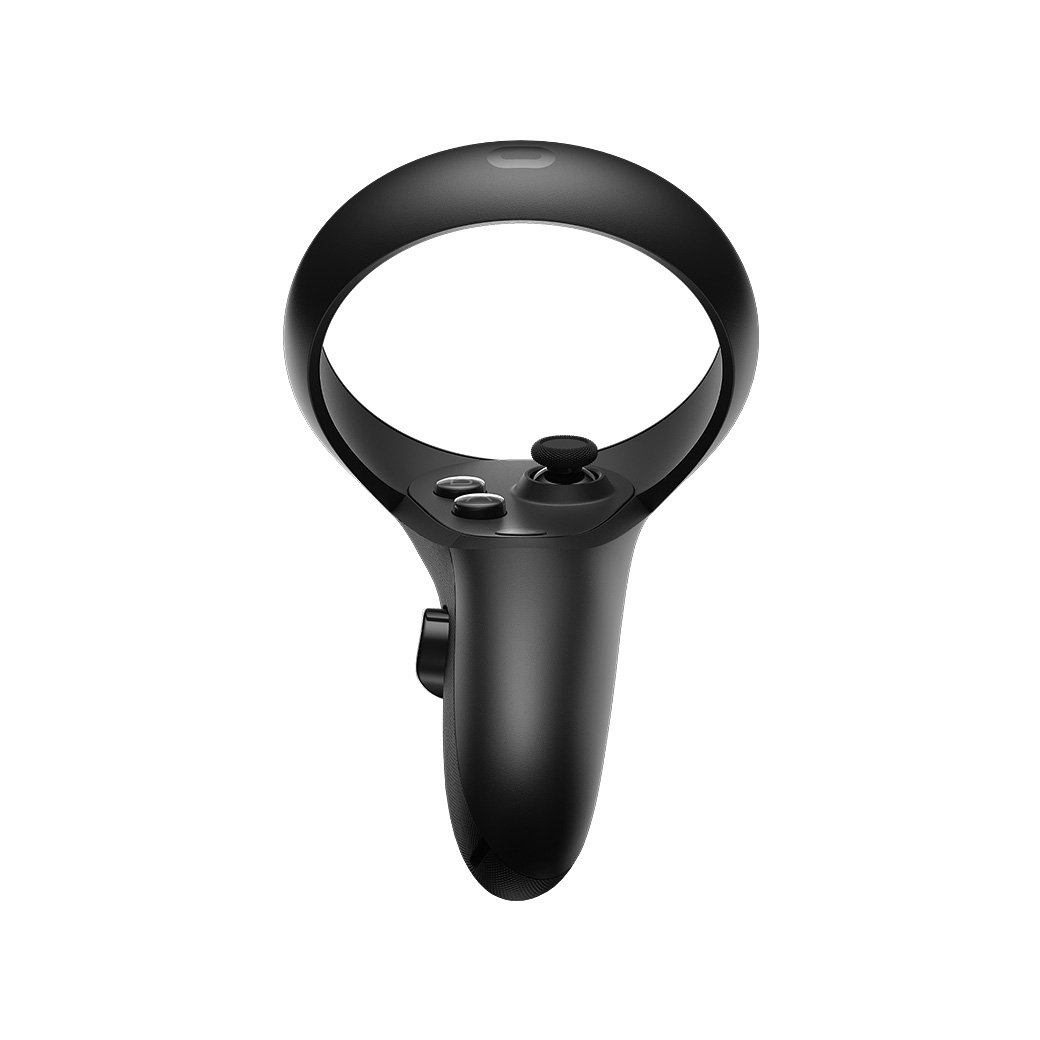
\includegraphics[width=\textwidth]{rift}
	\caption{Kontroler firmy Oculus~\cite{con1}}
	\label{fig:ctrlRift}
	\end{subfigure}
	~
	\begin{subfigure}[b]{0.45\textwidth}
	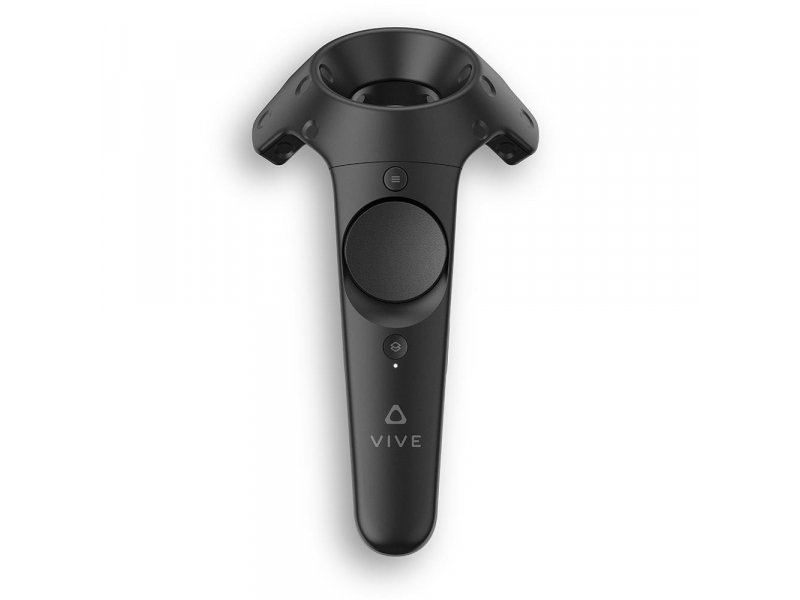
\includegraphics[width=\textwidth]{vive}
	\caption{Kontroler firmy Vive~\cite{con2}}
	\label{fig:ctrlVive}
	\end{subfigure}
\caption{Kontrolery VR}
\label{fig:kontrolery}
\end{figure}
Zapewniają one system śledzenia dłoni poprzez specjalne systemy - w przypadku Oculusa jest to system ukrytych diod, które emitują podczerwone światło, niewidoczne dla ludzkiego oka. Sensory które obserwują użytkownika analizują układ diod, dzięki czemu mogą przeanalizować pozycję. Analiza obrazu jest usprawniona poprzez przechowywania danych dotyczących położenia urządzenia na podstawie odczytów z żyroskopu, natomiast kierunek przemieszczenia na podstawie akcelerometru. W przypadku HTC Vive problem położenia rozwiązany jest bez przesyłania żadnych danych do obliczenia. W przeciwległych rogach pokoju montuje się tak zwane latarnie, które okresowo wysyłają wiązki światła podczerwonego, dzięki czemu na podstawie okresu pomiędzy odczytami z latarni, kontrolery są w stanie określić swoje położenie w przestrzeni. Problem rotacji jest rozwiązywany na podstawie żyroskopu tak jak jest to wykonywane w przypadku innych urządzeń. Oprócz tego nowsze urządzenia odchodzą od dodatkowych systemów śledzenia na rzecz wbudowanych kamer w zestawy do VR, ze względu na niechęć użytkowników do dodatkowych urządzeń które należy montować w celu poprawnego działania.~\cite{sledzenie, kontroleryDZB}.


\section{Wykorzystanie dłoni jako kontrolera}
\label{sec:historia}
	Jeżeli pomyśli się o świecie wirtualnym oraz jego celu, czyli stworzeniu realnych i naturalnych doznań, wydaje się naturalnym używanie dłoni w celu interakcji ze sceną, bez konieczności trzymania dodatkowych kontrolerów. I rzeczywiście podejście to było też zastosowane w praktyce. Użycie dłoni, a konkretnie rękawicy na dłoniach jako kontrolera w świecie wirtualnym po raz pierwszy wykorzystano w 1977 roku przez Dana Sandina. Dzięki wykorzystaniu światłoczułych czujników na każdym z palców, możliwe było otrzymanie pomiarów zgięcia palców, które głównie służyło do regulacji suwaków~\cite{sayreGlove}. Współczesne rękawice znacznie się rozwinęły od tamtej pory, implementując różnorodność rozwiązań. W celu ustalenia orientacji urządzenia korzystają przynajmniej z jednej jednostki do pomiaru inercji, stosując dokładne filtry w celu jak największej dokładności. Wiele urządzeń korzysta z wielu takich jednostek pomiarowych, umieszczając po dwie bądź trzy na każdym palcu w celu dokładnego mierzenia pozycji palców. Oprócz tego urządzenia stosują systemy wibracji, zwiększając tym samym jak realistyczne jest doznanie, w szczególności gdy dochodzi do interakcji z przedmiotami. Rękawice są dobrze znane w branży wirtualnej rzeczywistości. Rozwiązania te jednak pozostają drogie i nie tak dokładne jak prezentowane w sekcji~\ref{sec:kontroleryVR} przykładowe kontrolery, w szczególności braku uniwersalnego braku rozwiązania dla wszystkich użytkowników - nie każdy w końcu ma dłoń tej samej wielkości. Problemy takie jak ten próbowała rozwiązać firma \textit{Plexus} która w swoim rozwiązaniu stosuje regulowanej długości nakładki na palce, jednak produkt ten nie jest jeszcze dostępny na rynku~\cite{plexus}. Z pewnością można się spodziewać rozwoju tego i wielu innych produktów, i jak to bywa z wieloma początkowo drogimi technologiami - spadku cen gdy zainteresowanie produktem stanie się większe. Na chwilę obecną widać duże zainteresowanie tego rodzaju rozwiązaniami i wiele osób już wykorzystuje tego rodzaju produkty w biznesie - w rozwój technologi inwestują takie firmy jak: Toyota, Netflix, Audi czy NASA. Biorąc to pod uwagę nie można zaniedbać potencjału jaki się kryje w tym segmencie rynku wirtualnej rzeczywistości~\cite{manus}.
	
	
	
	
	
	
	
	
	
	
	
	
	
	
	
	
	
	
	
	
